\tikzset{every picture/.style={line width=0.9pt}}
\begin{tikzpicture}
	% First image
	\node[anchor=north west] (image1) at (0,0) {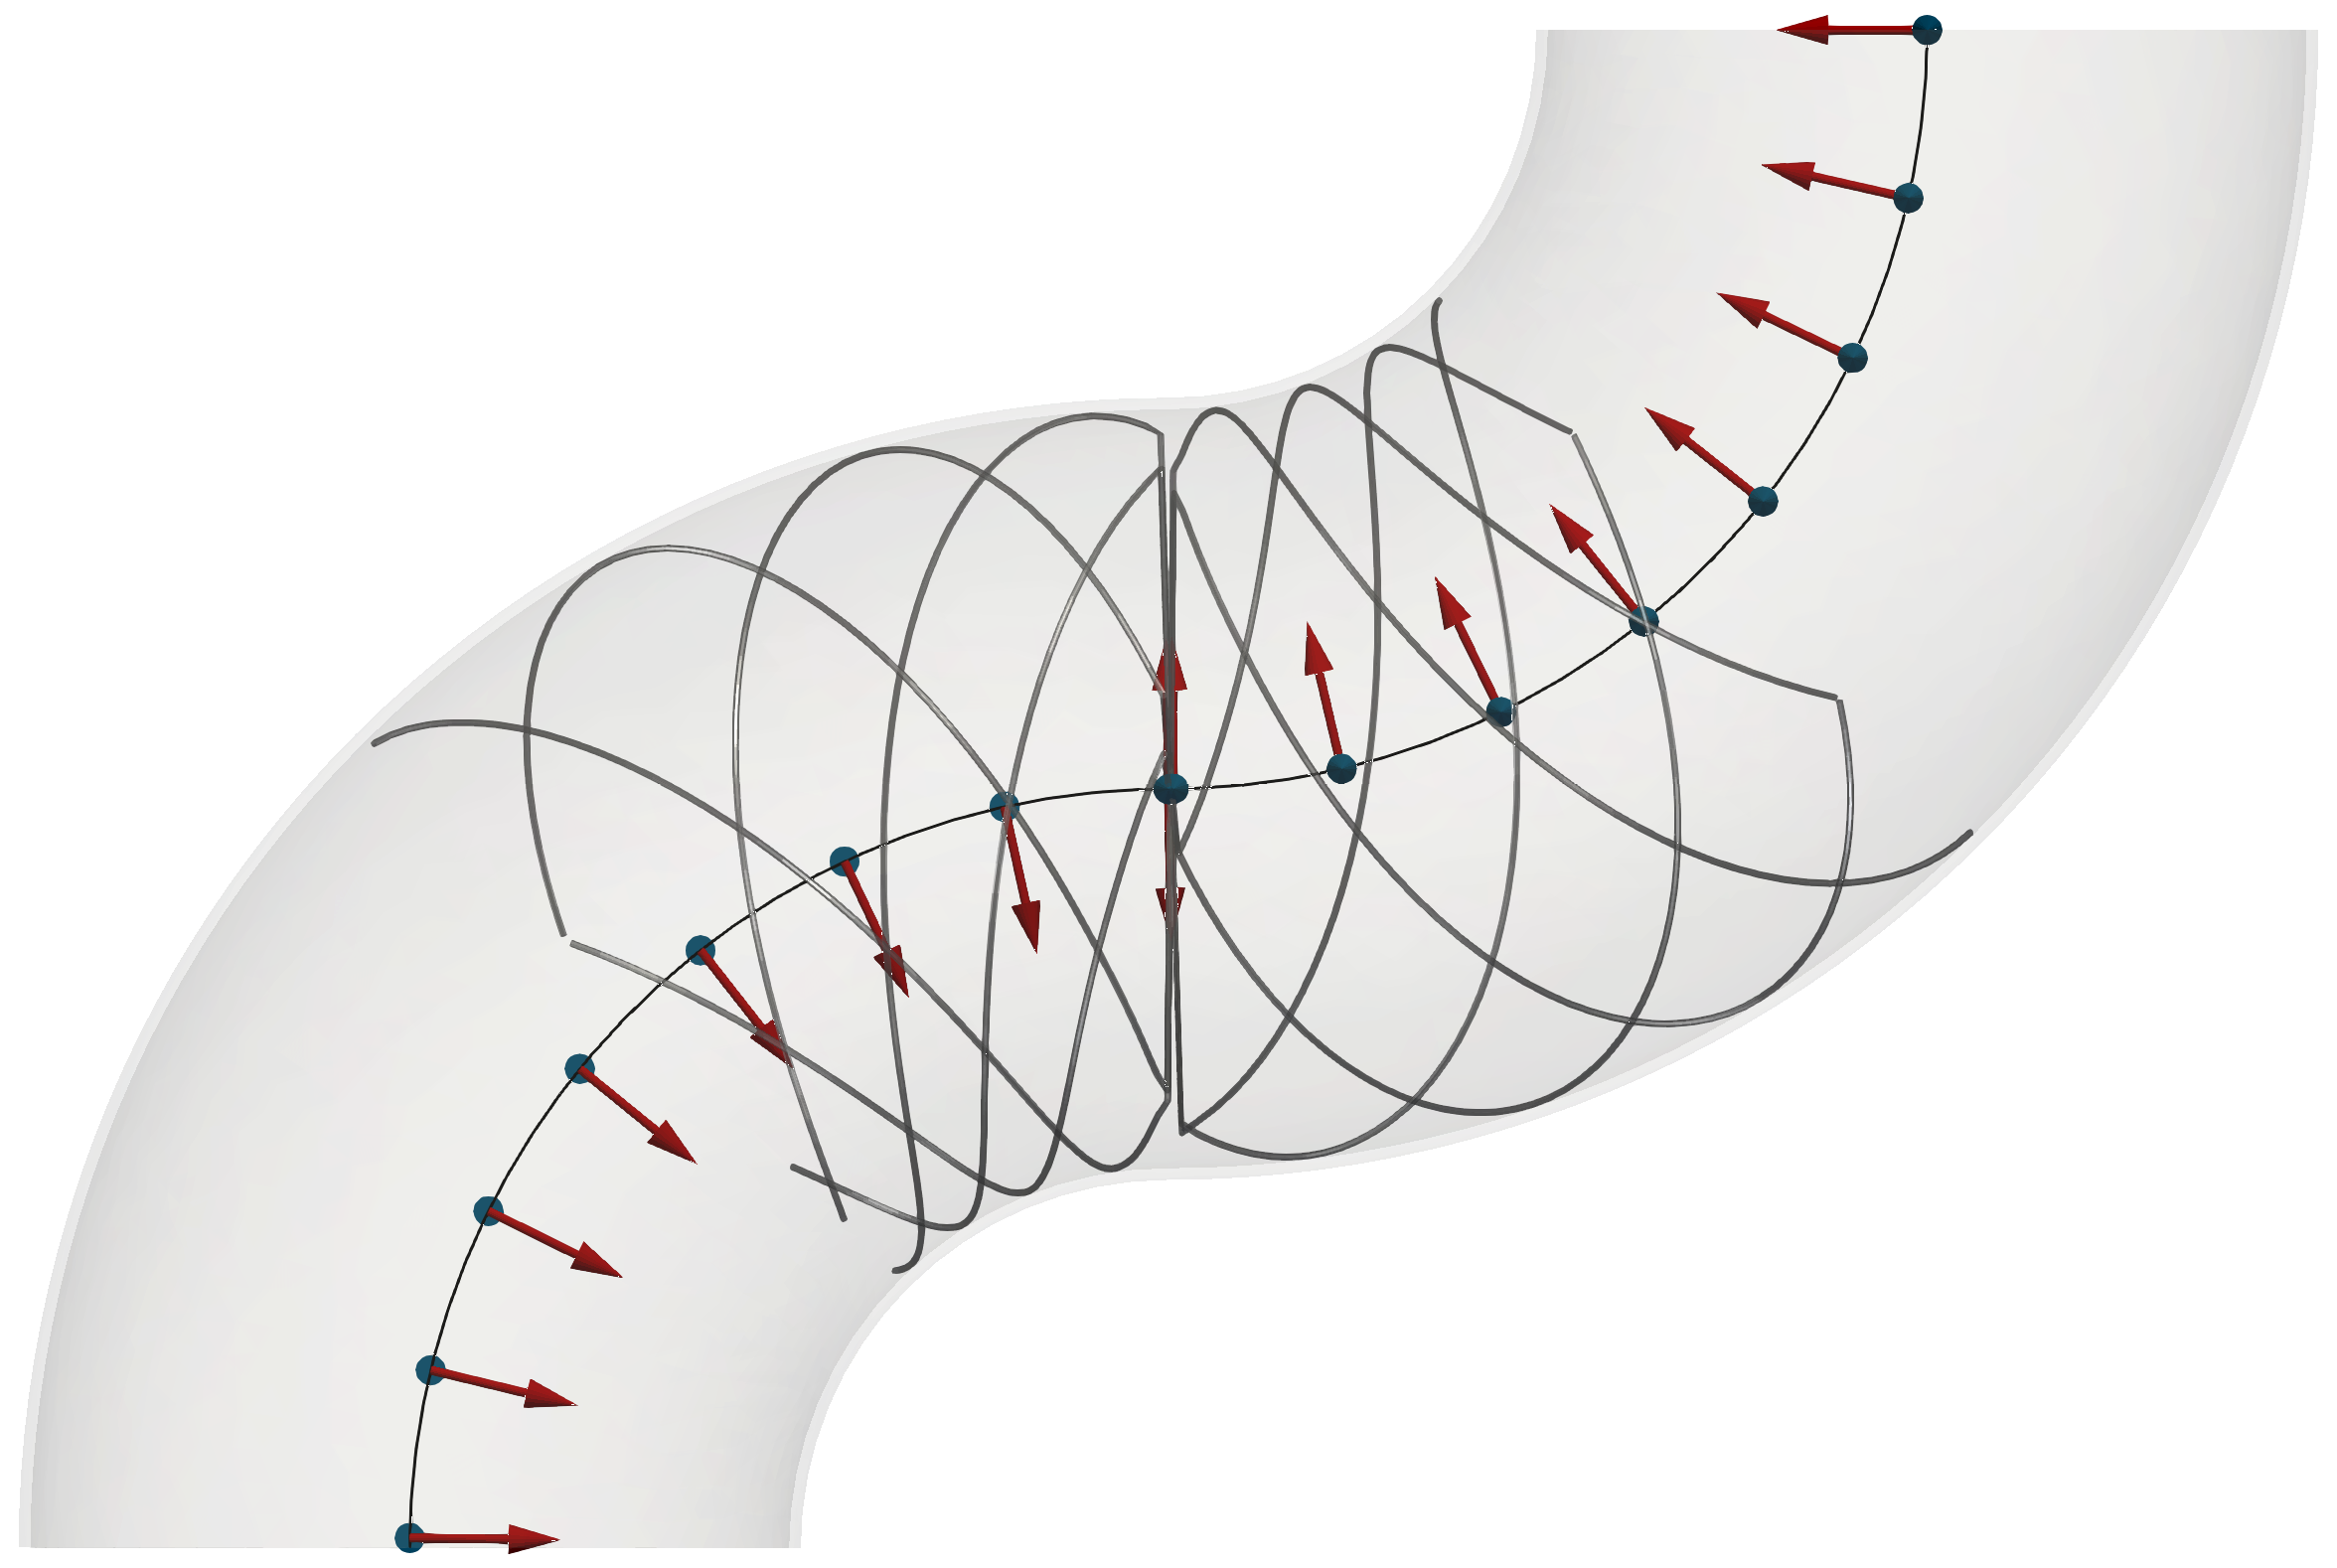
\includegraphics[width=0.425\linewidth]{chapter4/Figures/Coordinate_System/Coordinate_System_Cross_Section_FAIL.png}};
	\node[below=of image1, yshift=1cm] (eq1) {
		\begin{minipage}[l]{0.425\textwidth}
			\begin{equation}
				\begin{split}
					\vec{e}_T &= \vec{T}\\
					\vec{e}_1 &= \vec{R} / R\\
					\vec{e}_2 &= \vec{e}_T \times \vec{e}_1 \\
				\end{split}
				\label{eqn:frenet}
			\end{equation}
		\end{minipage}
	};

	% Second image
	\node[anchor=north west] (image2) at ([xshift=1cm]image1.north east) {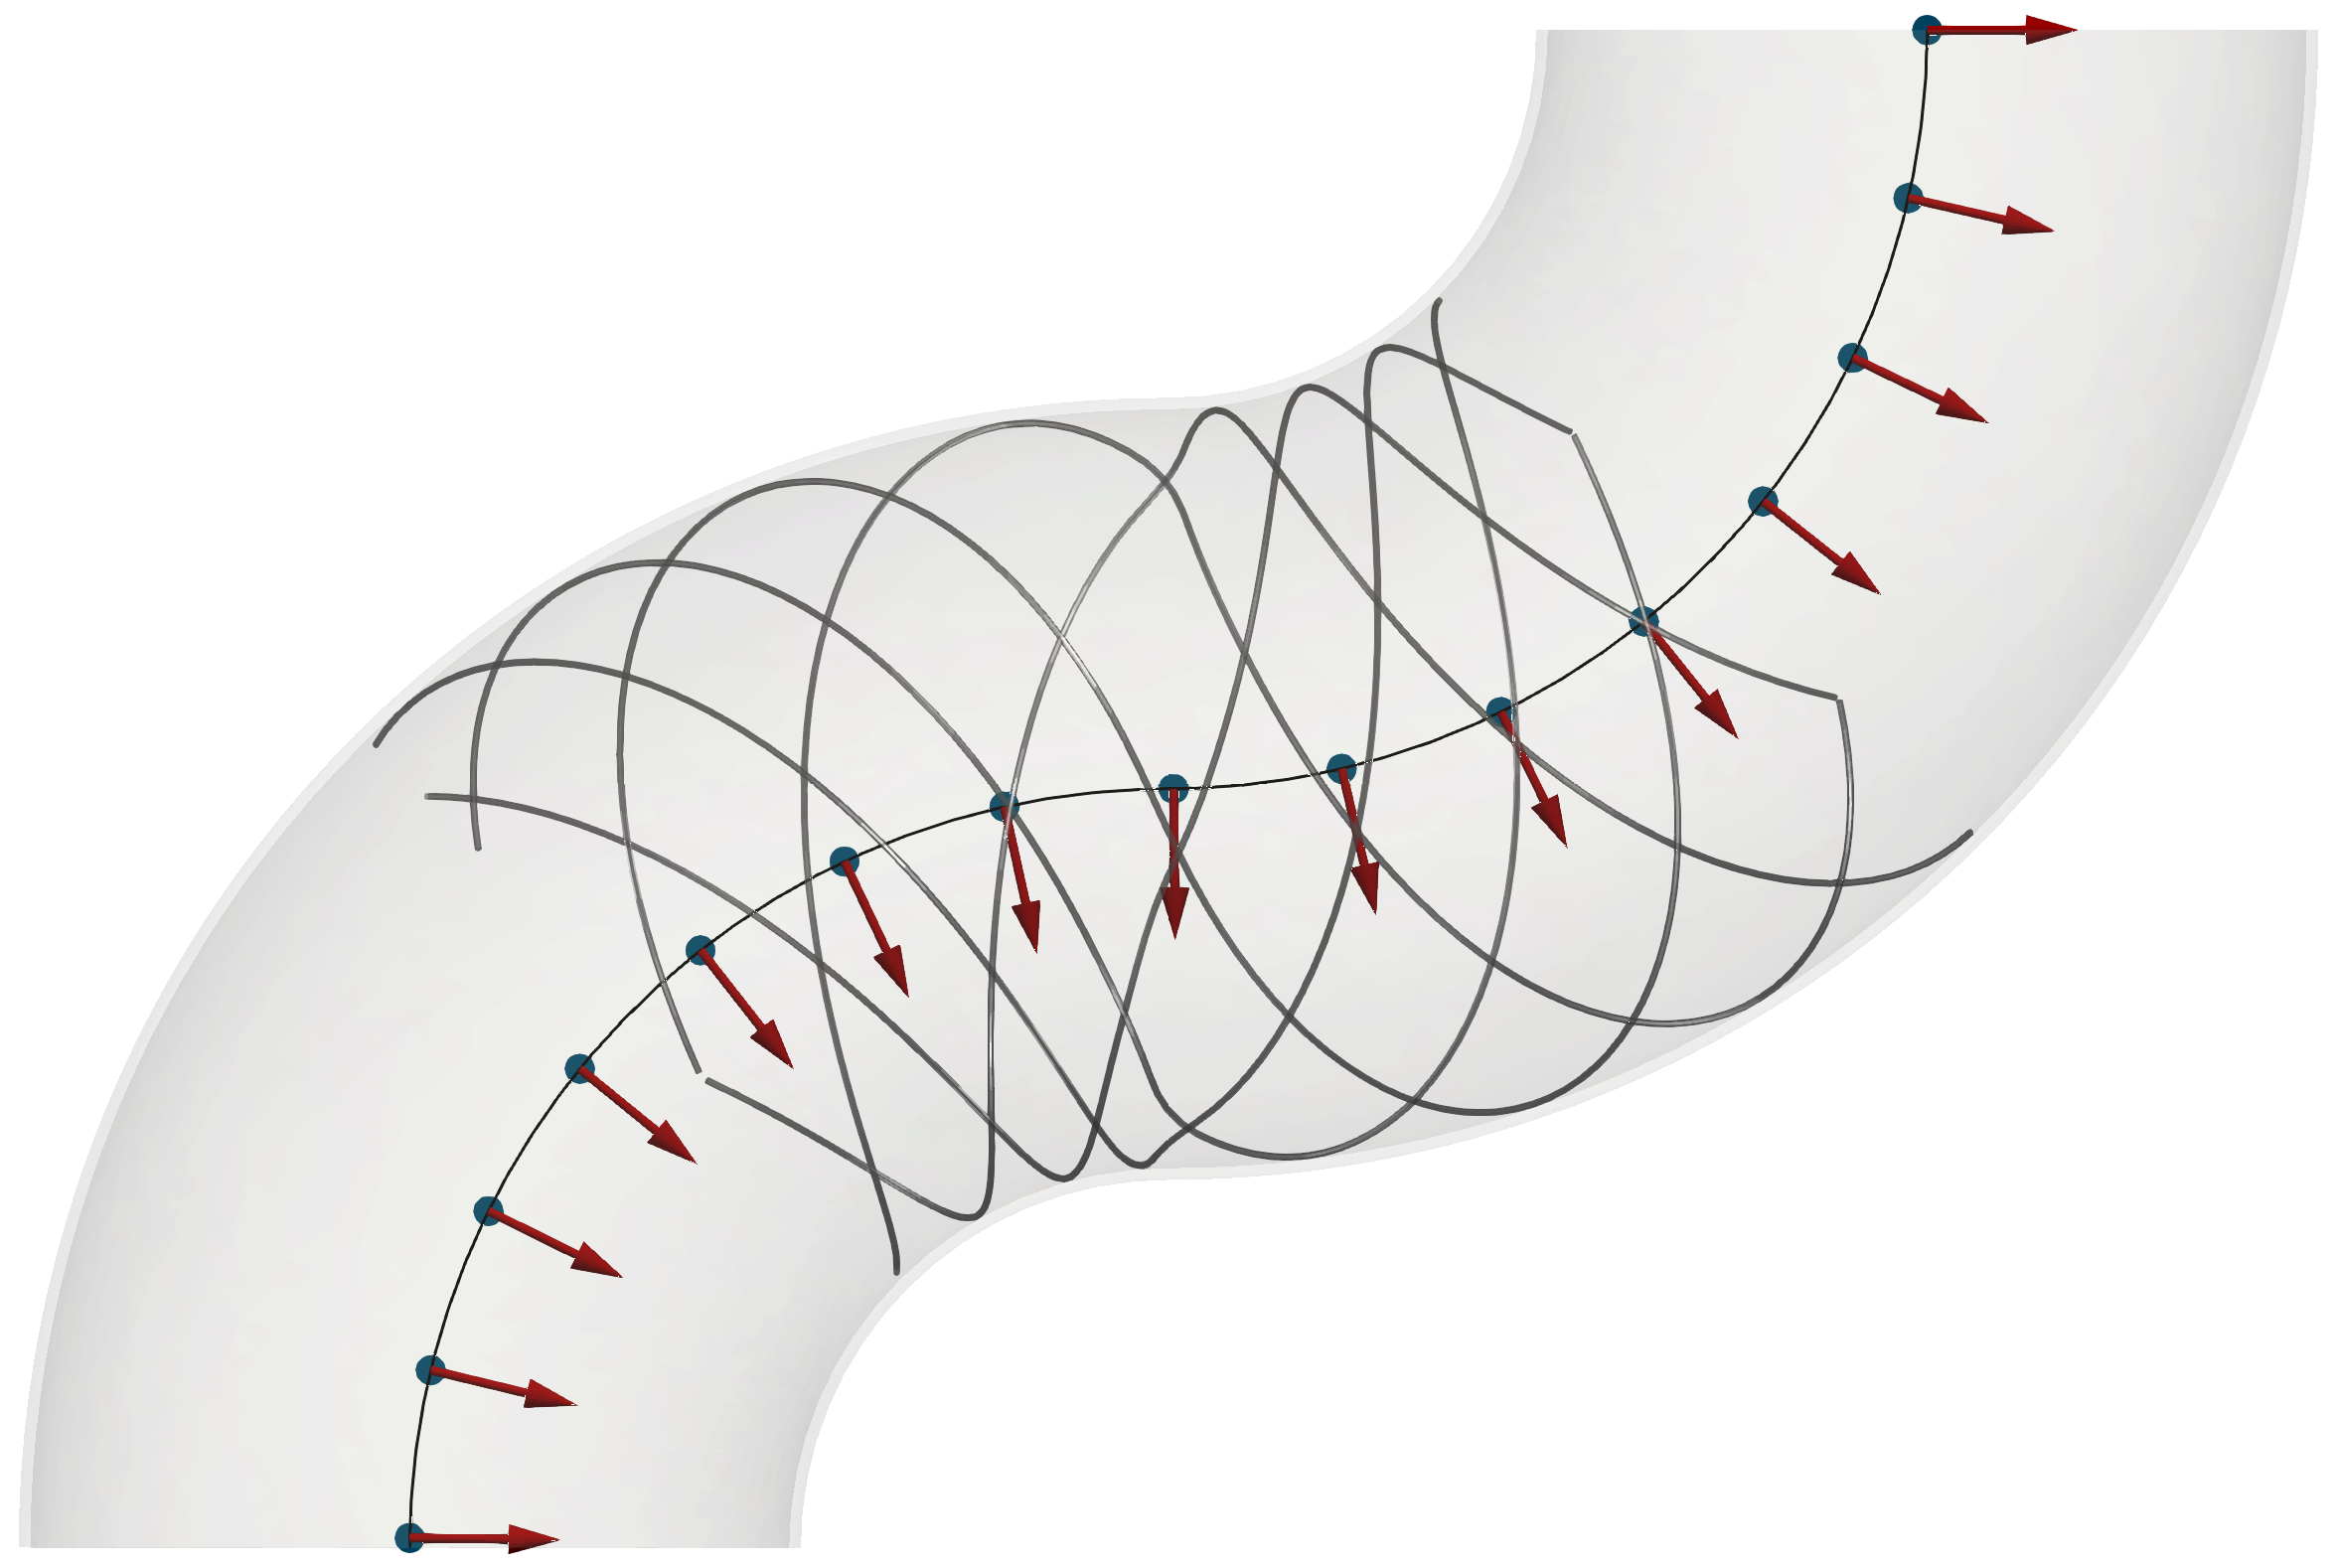
\includegraphics[width=0.425\linewidth]{chapter4/Figures/Coordinate_System/Coordinate_System_Cross_Section.png}};;
	\node[below=of image2, yshift=1cm] (eq2) {\begin{minipage}[l]{0.425\textwidth}
			\begin{equation}
				\begin{split}
					\vec{e}_T &= \vec{T}\\
					\vec{e}_1 &= \text{RMF}\\
					\vec{e}_2 &= \vec{e}_T \times \vec{e}_1 \\
				\end{split}
				\label{eqn:coordinate_sys}
			\end{equation}\hfill
		\end{minipage}};
\end{tikzpicture}
